\chapter{DEPLOYMENT}

\section{Folder Structure}
The deployed College Event Management System (Planova) utilizes the standard Laravel directory structure, optimized for server environments. The project is organized to separate public-facing assets from core backend logic securely.

\begin{figure}[H]
    \centering
    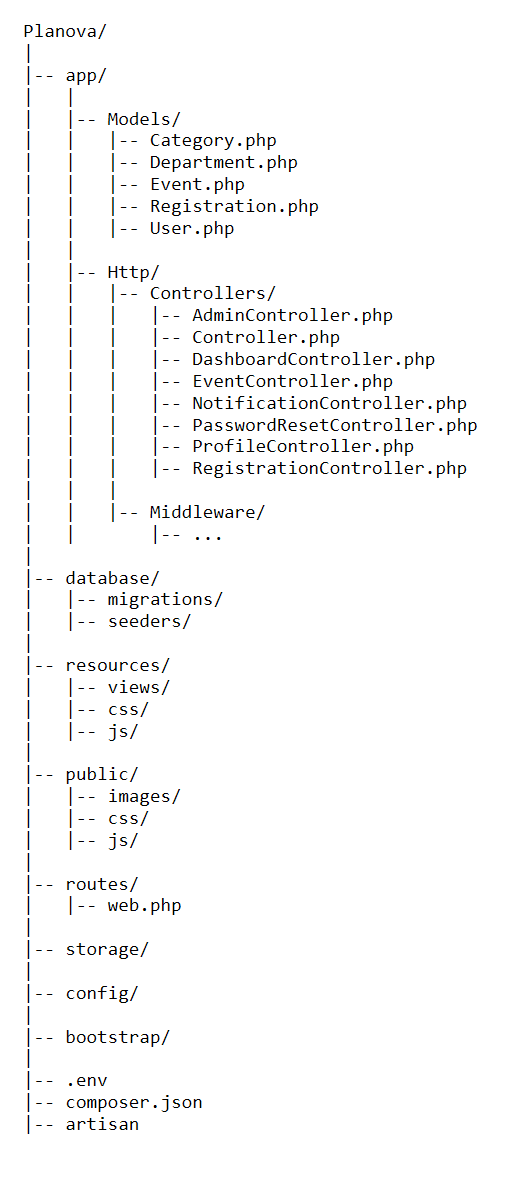
\includegraphics[width=0.6\textwidth]{deployment_tree.png}
    \caption{Planova File and Folder Structure}
    \label{fig:deployment_tree}
\end{figure}

\section{Hosting Environment}
The system is deployed on a standard web server stack operating on Apache or Nginx, PHP 8.2+, and MySQL/MariaDB. For security purposes, the web server's "Document Root" is exclusively pointed towards the \texttt{public/} directory. This prevents end-users from accessing core application files, configuration settings, and the \texttt{.env} file containing database credentials.